\begin{frame}[t]{Die Messbruecke - Modellierung eines variablen Widerstandes}

  \begin{spacing}{0.9} \begin{tiny}
      \begin{table}[h!]
        \begin{tabular}{p{10cm}}
          \hline
          \textbf{Das Messprinzip} \\
          \hline                   \\
          \begin{minipage}{\textwidth}

            Ist eine Messbruecke abgegleichen, so gilt:
            \begin{equation}
              \frac{R_1}{R_2} = \frac{R_3}{R_4}
            \end{equation}
            \begin{equation}
              V_{AB} = 0
            \end{equation}
            Um die Temperatur messen zu können, ersetzen wir den Widerstand $R_2$ durch einen PTC.\newline
            Verändert sich der $R_2$ ist die Brücke nicht mehr abgegleichen und die Spannung $V_{AB}$ ungleich 0.
            \begin{figure}
              \scalebox{0.6}{
                \centering
                \begin{circuitikz}
                  \ctikzset{bipoles/thickness=1}
                  \ctikzset{bipoles/length=.6cm}
                  \draw
                  (0,0) to [short, *-] (4,0)
                  (0,0) to [V, l_=$V_{1}$] (0,-4)
                  (2,0) to (2,-0.5)
                  (4,0) to (4,-0.5)
                  (2,-0.5) to [R, l_=$R_{1}$] (2,-1.5);
                  \ctikzset{resistors/fill=red}
                  \draw
                  (2,-2.5) to [thRp, l_=$R_{2}$] (2,-3.5);
                  \ctikzset{resistors/fill=none}
                  \draw
                  (2,-1.5) to (2,-2.5)
                  (2,-2) to [short,*-o] (2.25,-2) node[right]{$V_{a}$}
                  (4,-1.5) to (4,-2.5)
                  (4,-2) to [short,*-o] (4.25,-2) node[right]{$V_{b}$}
                  (4,-0.5) to [R, l_=$R_{3}$] (4,-1.5)
                  (4,-2.5) to [R, l_=$R_{4}$] (4,-3.5)
                  (2,-3.5) to (2,-4)
                  (4,-3.5) to (4,-4)
                  (0,-4) node[ground]{}
                  (2,-4) node[ground]{}
                  (4,-4) node[ground]{}
                  ;
                \end{circuitikz}
              }

            \end{figure}
            Um dieses Prinzip zu simulieren werden wir nun in LTspice den Widerstand $R_2$ modellieren und variieren.
          \end{minipage}
          \\
        \end{tabular}

      \end{table}

    \end{tiny} \end{spacing}

\end{frame}

\begin{frame}[t]{Die Messbruecke - Modellierung eines variablen Widerstandes}

  \begin{spacing}{0.9} \begin{tiny}
      \begin{table}[h!]
        \begin{tabular}{p{10cm}}
          \hline
          \textbf{Ansatz}               \\
          \hline                        \\
          \begin{minipage}{\textwidth}
            \begin{itemize}
              \item Der Widerstand soll durch einen PTC ersetzt werden
              \item Wir nehmen zunächst vereinfacht an, dass sich der Widerstand zwischen 0$°$C - 100$°$C von 1.5k$\Omega$ linear auf 3.5k$\Omega$ erhöht.
            \end{itemize}
          \end{minipage}
          \\
          \\
          \hline
          \textbf{Variablen in LTspice} \\
          \hline                        \\
          \begin{minipage}{\textwidth}
            \begin{figure}
              \centering
              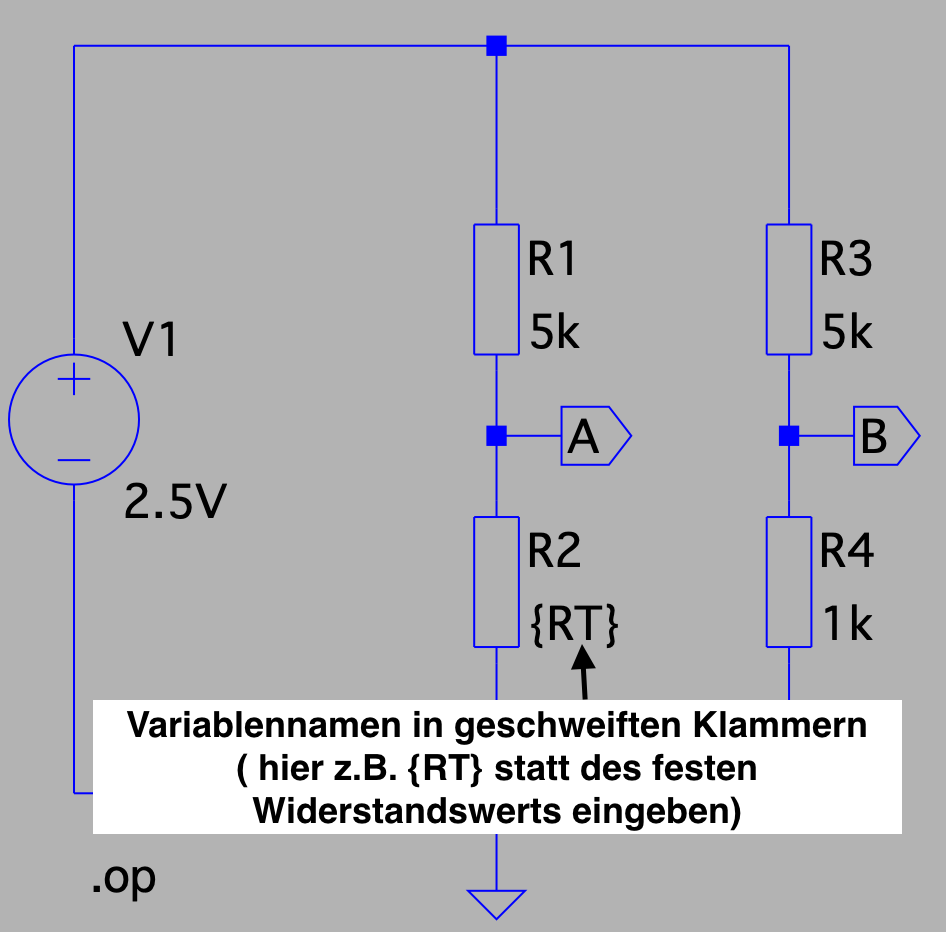
\includegraphics[width=0.45\linewidth]{pictures/rt_var.png}
            \end{figure}
          \end{minipage}
          \\
        \end{tabular}

      \end{table}

    \end{tiny} \end{spacing}

\end{frame}

\begin{frame}[t]{Die Messbruecke - Modellierung eines variablen Widerstandes}
  \begin{spacing}{0.9} \begin{tiny}
      \begin{table}[h!]
        \begin{tabular}{p{3cm} p{7cm}}
          \hline
          \textbf{Definition von Variablen} \\
          \hline                            \\
          \begin{minipage}{.3\textwidth}
            \begin{figure}
              \centering
              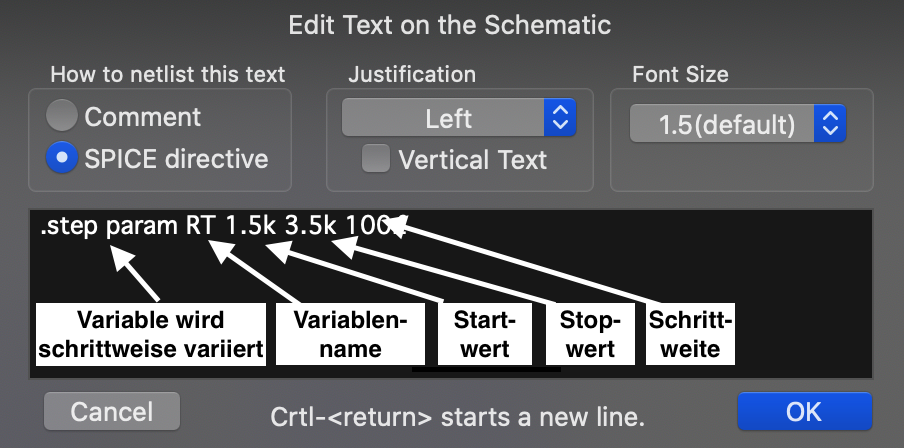
\includegraphics[width=0.9\linewidth]{pictures/step_param.png}
            \end{figure}
          \end{minipage}
           &
          \begin{minipage}{.7\textwidth}
            Variablen können auf verschiedene Weisen variiert werden.\newline
            \begin{itemize}
              \item Eine Möglichkeit ist die spice-Direktive $.step\ param$
              \item Fügt einfach eine spice-Direktive hinzu\newline (Edit $->$ Spice Directive (\textbf{oder drückt S}))
              \item $.step\ param\ <varname> <start> <stop> <step>$
            \end{itemize}
          \end{minipage}
          \\
        \end{tabular}
        \\
        \begin{tabular}{p{5cm} p{5cm}}
          \hline
          \textbf{Simulieren in Abhängigkeit von RT} \\
          \hline                                     \\
          \begin{minipage}{0.5\textwidth}
            \begin{figure}
              \centering
              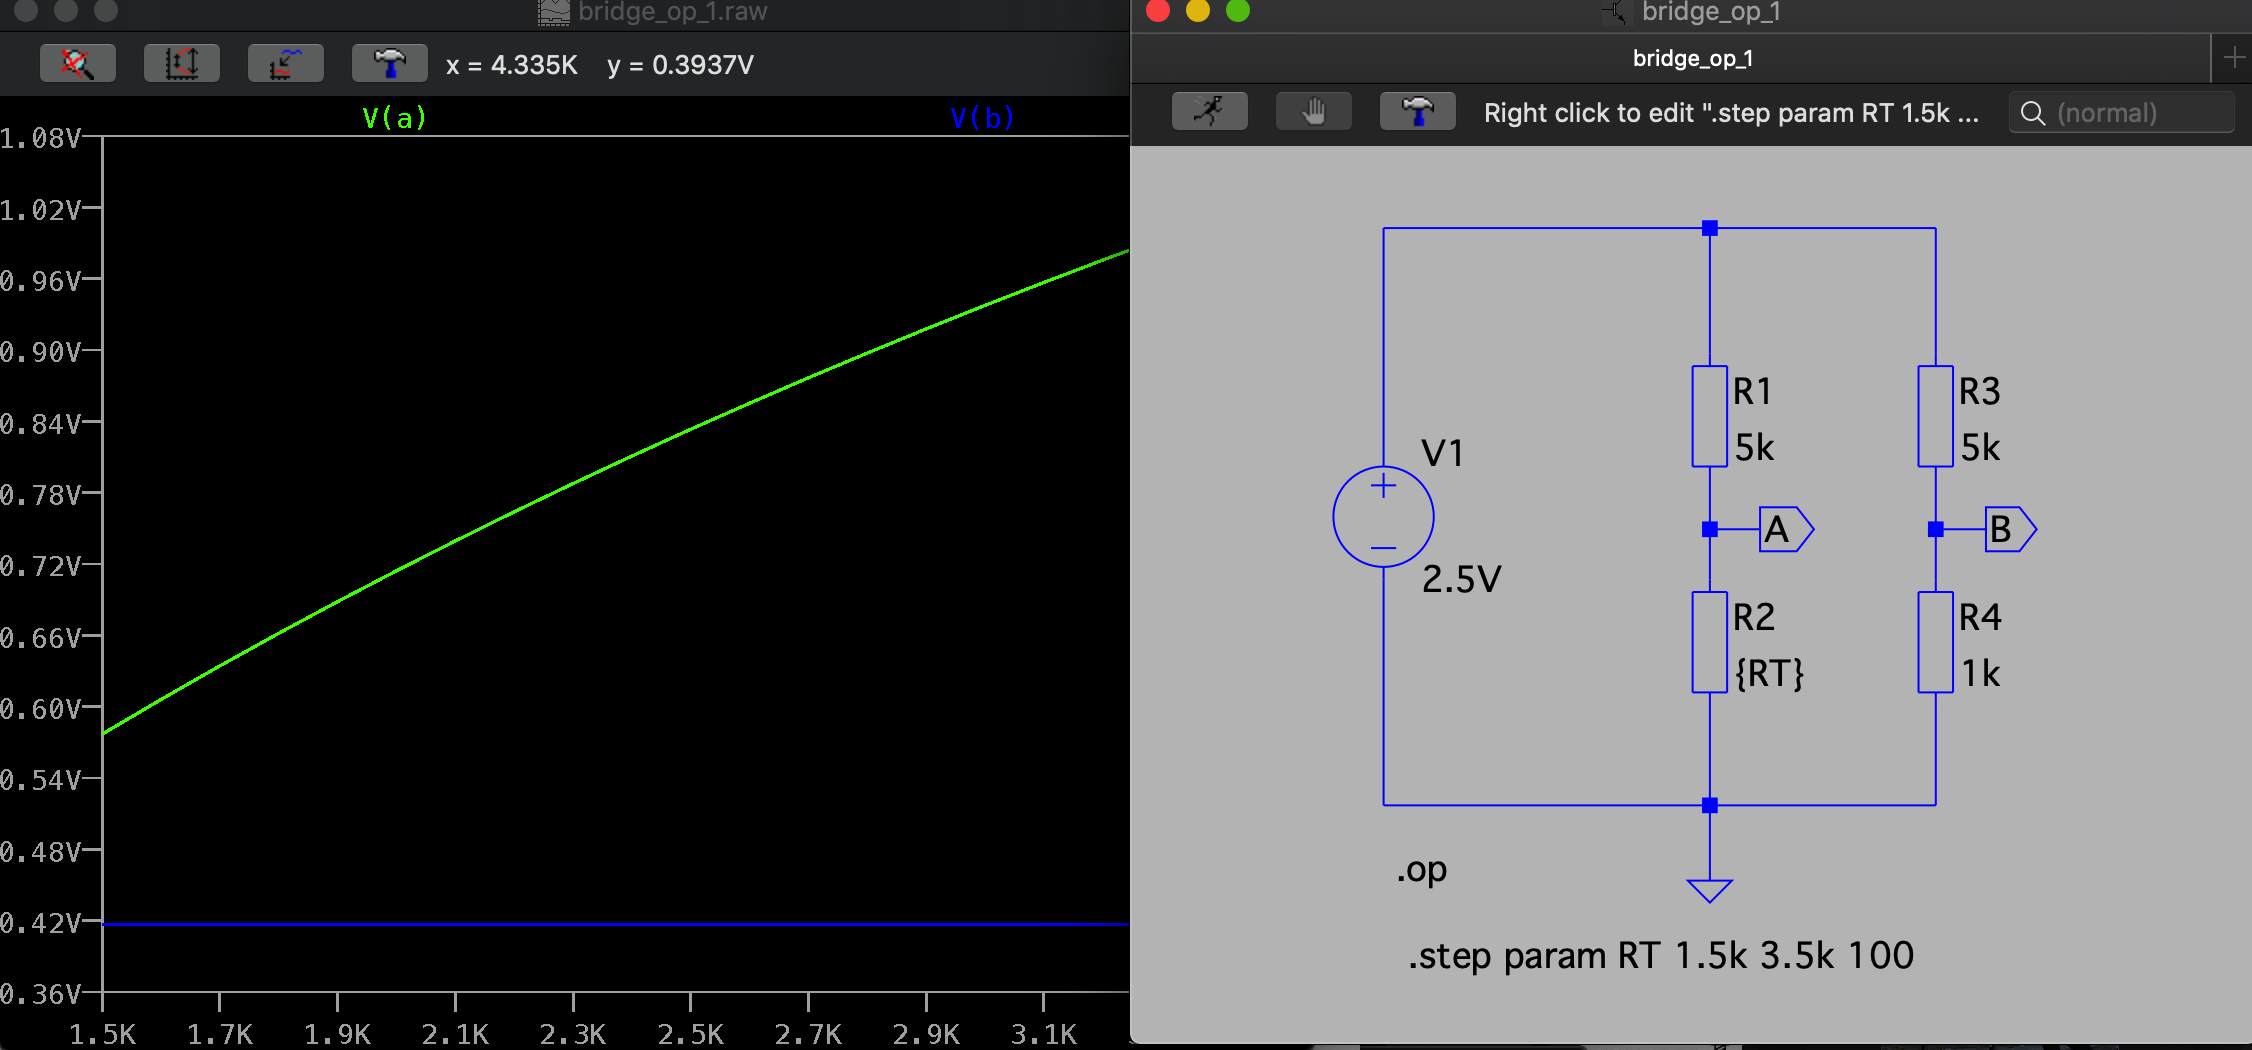
\includegraphics[width=0.9\linewidth]{pictures/rt_analysis_1.png}
              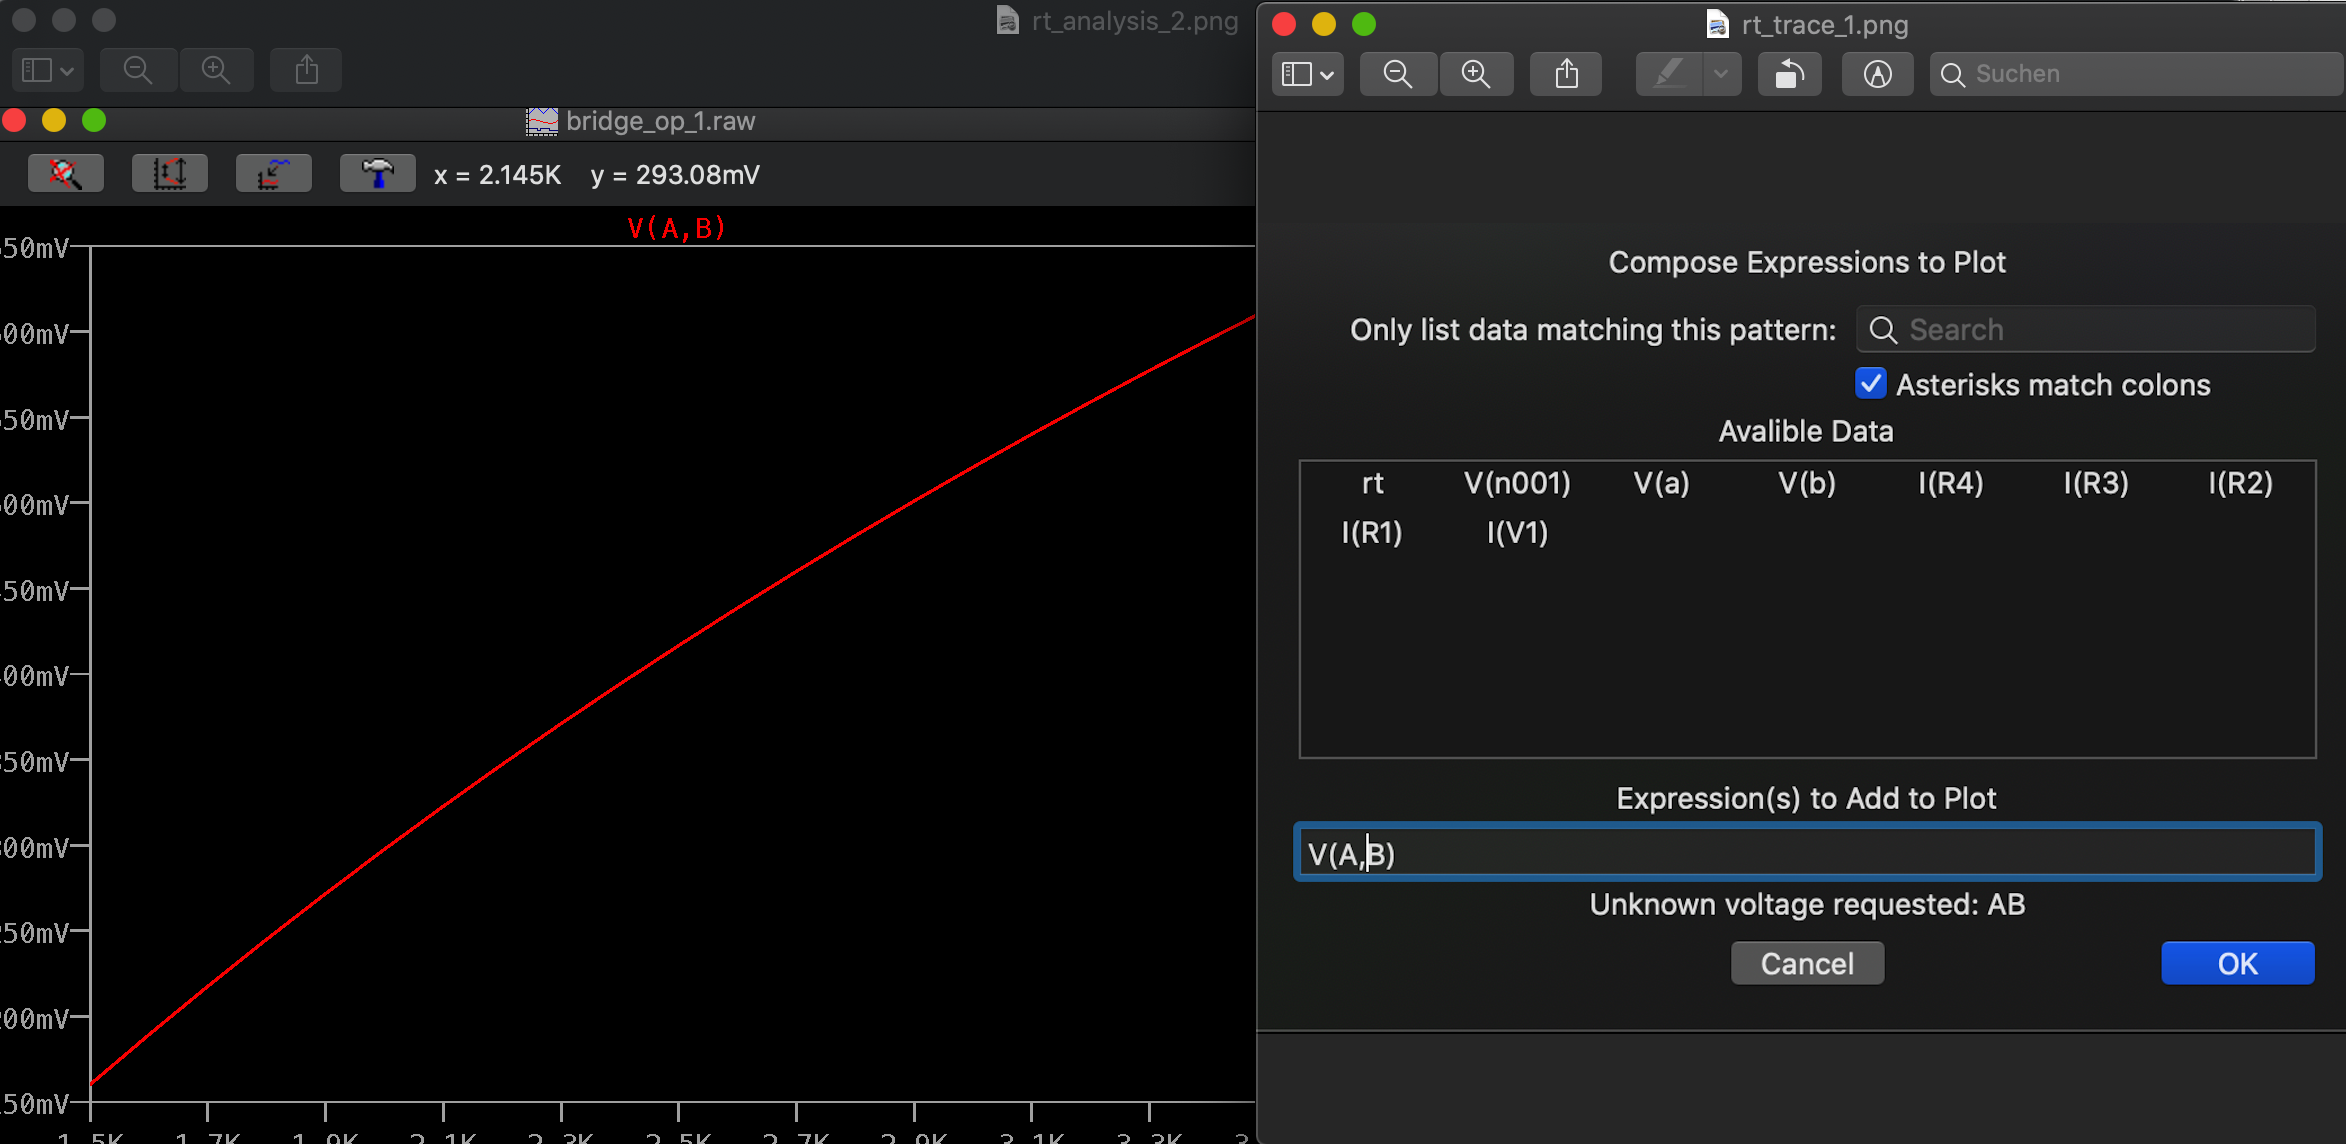
\includegraphics[width=0.9\linewidth]{pictures/rt_analysis_3.png}
            \end{figure}
          \end{minipage}
           &
          \begin{minipage}{0.5\textwidth}
            \begin{itemize}
              \item Es wird die \textbf{Spannung} über dem variablen Widerstand auf der x-Achse aufgetragen
              \item Ihr könnt die Spannung zwischen den $A$ und $B$ anzeigen lassen:
              \item ... über den waveform viewer $->$ add traces $->$ V(A,B) (Spannung von Knoten zu Knoten)
              \item ... im schematic, indem ihr mit der roten Messpitze (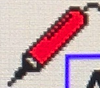
\includegraphics[scale=0.1]{pictures/rot.png}) auf ein Potential klickt,
              \item ...... die linke Maustaste gedrückt haltet und mit der erscheinenden schwarzen Messpitze (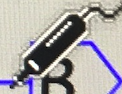
\includegraphics[scale=0.1]{pictures/black.png}) auf der zweite Potential klickt.
              \item Der \textbf{Strom} kann angezeigt werden, indem ihr mit der Maus über ein Bauteil fahrt und die Strommesszange (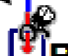
\includegraphics[scale=0.1]{pictures/current.png}) anklickt.
              \item Die \textbf{Verlustleistung} kann angezeigt werden, indem ihr mit der Maus über ein Bauteil fahrt, \textbf{Shift} gedrückt haltet und das Temperatursymbol (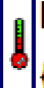
\includegraphics[scale=0.1]{pictures/power.png}) anklickt.
            \end{itemize}
          \end{minipage}
          \\
        \end{tabular}

      \end{table}
    \end{tiny} \end{spacing}
\end{frame}

\begin{frame}[t]{Die Messbruecke - Modellierung eines variablen Widerstandes}

  \begin{spacing}{0.9} \begin{tiny}
      \begin{table}[h!]
        \begin{tabular}{p{10cm}}
          \hline
          \textbf{Formeln visualisieren} \\
          \hline                         \\
          \begin{minipage}{\textwidth}
            Weiterhin könnt ihr im waveform viewer auch beliebige Formlen und somit Kennwerte
            eurer Schaltung berechnen und visualisieren.
            \begin{figure}
              \centering
              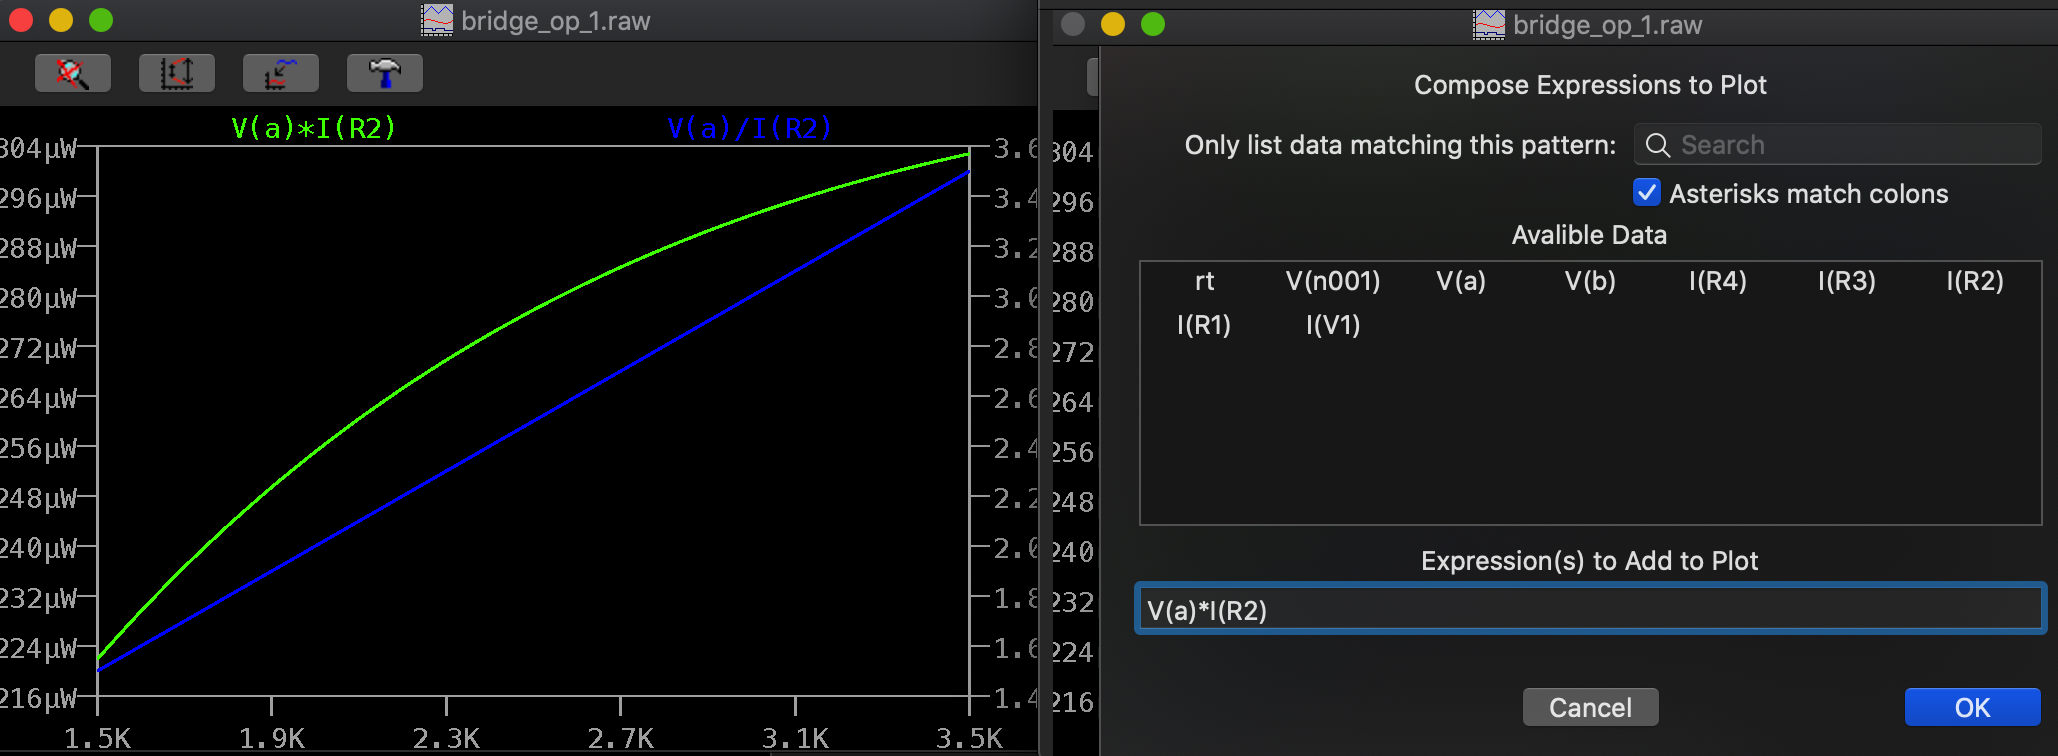
\includegraphics[width=0.95\linewidth]{pictures/waveform_formulas.png}
            \end{figure}
            Ihr solltet die folgenden Messwerte der Brückenschaltung ermitteln, bzw. ermittelt haben:
            \begin{itemize}
              \item Brückenspannung $V_{AB}$
              \item Strom durch $I(R_2)$
              \item Verlustleistung $P(R_2)=V_aI(R_2)$
              \item Verifiziert den Widerstandswert $R_2=\frac{V(a)}{I(R_2)}$
            \end{itemize}
          \end{minipage}
          \\
        \end{tabular}

      \end{table}

    \end{tiny} \end{spacing}

\end{frame}
